\documentclass[a4paper, 12pt]{article}
\usepackage{csquotes}
\usepackage{titlesec}
\usepackage[ngerman]{babel}
\usepackage[a4paper, left=3cm, right=3cm, top=2cm, bottom=2cm]{geometry}
\usepackage{fouriernc}
\usepackage{titlesec}
\usepackage{keystroke}

\newcommand{\makeTitleAndTable}{
    \begin{titlepage}
        \centering
        \vspace*{1.5cm}
        {\Huge Einfacher SPH Flüssigkeitssimulator mit Beschleunigter Nachbarschaftssuche\par}
        \vspace{1cm}
        {\LARGE Thierry Meiers\par}
        {\Large Bachelor Projekt\par}
        \begin{figure}[H]
            \centering
            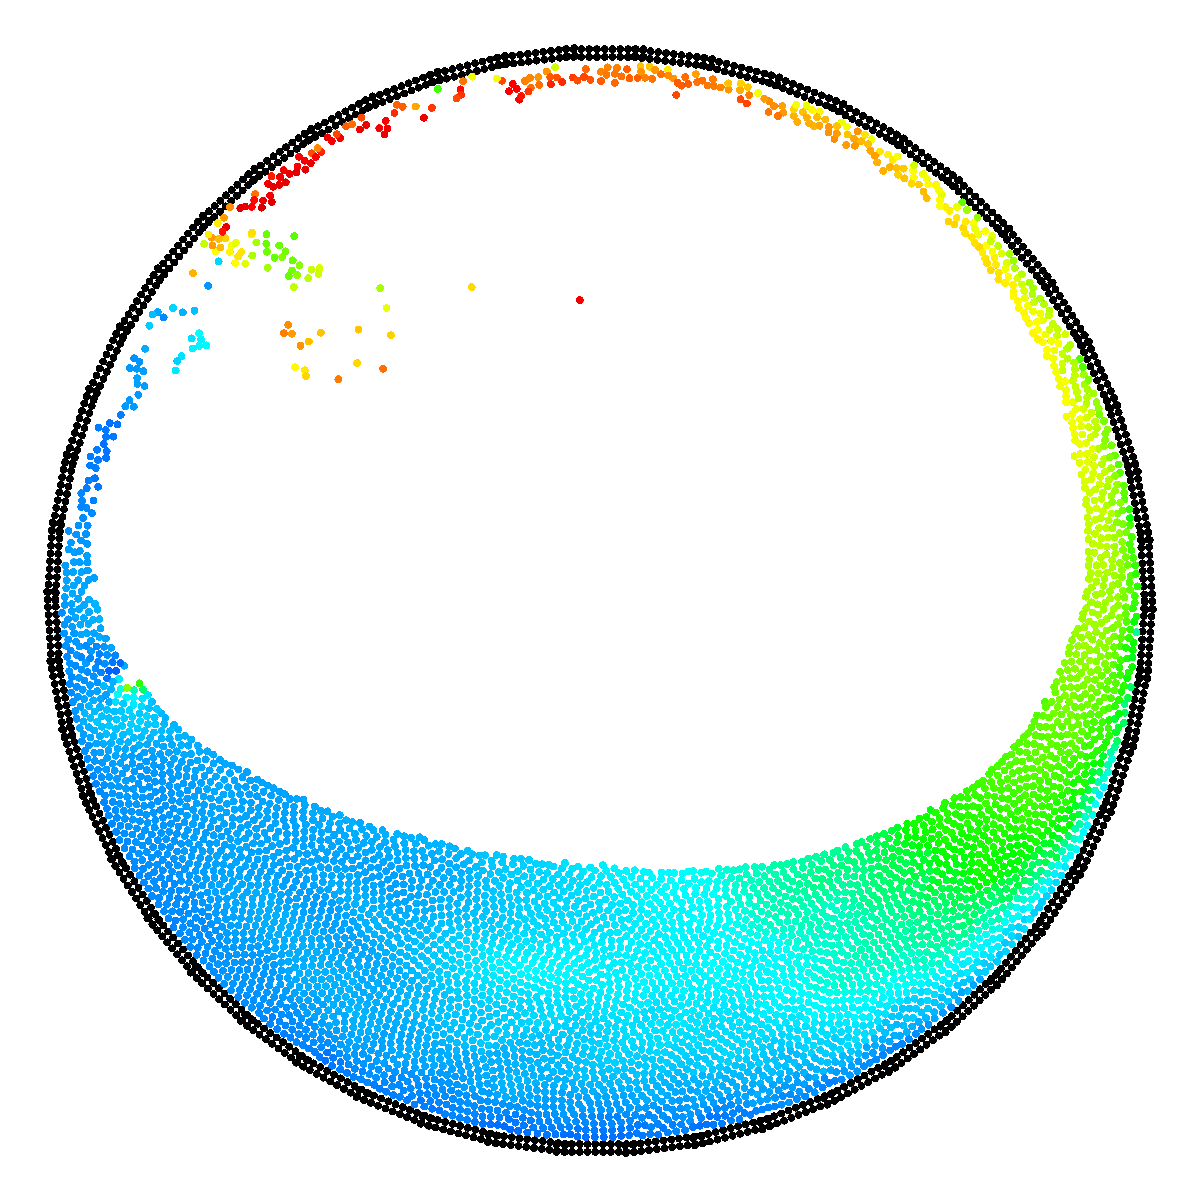
\includegraphics[width=.7\textwidth]{graphics/FirstPage.png}
        \end{figure}
        \vspace{0.5cm}
        {\large Albert-Ludwigs-Universität Freiburg\\Technische Fakultät\\Graphische Datenverarbeitung\par}
        \vfill
        {\large \today \par}
    \end{titlepage}
    \pagenumbering{gobble}
    \tableofcontents
    \clearpage
    \pagenumbering{arabic}
}

\usepackage[ngerman]{babel}
\usepackage[dvipsnames]{xcolor}
\usepackage{graphicx} 
\usepackage{microtype}
\usepackage{float}
\usepackage{parskip}
\usepackage{amsmath}
\usepackage{hyperref}
\usepackage{enumitem}
\usepackage{dsfont}
\usepackage{algorithm}
\usepackage{float}
\usepackage[noend]{algpseudocode}
\usepackage{menukeys}
\usepackage{subfigure}
\usepackage{wrapfig}

\makeatletter
\def\BState{\State\hskip-\ALG@thistlm}
\makeatother

\setcounter{tocdepth}{2}
\begin{document}

\makeTitleAndTable

\section{Einführung}
Fluidsimulationen haben sich zu einem unverzichtbaren Werkzeug in zahlreichen Bereichen unserer Gesellschaft entwickelt. Sie ermöglichen die präzise Simulation von Flüssigkeiten und Gasen in verschiedenen Umgebungen, wodurch das Verhalten dieser Stoffe und ihre Interaktionen mit der Umgebung untersucht werden können. Aufgrund ihrer Vielseitigkeit kommen Fluidsimulationen in einer großen Bandbreite von Anwendungsgebieten zum Einsatz, darunter die Optimierung von Fahrzeugen und Gebäuden, Wettervorhersagen, medizinische Forschung, die Erzeugung realistischer Effekte in Filmen und Spielen, industrielle Prozesse, Energieerzeugung und die Entwicklung von Sportgeräten. Diese Simulationen tragen wesentlich dazu bei, Designs zu verbessern, die Effizienz zu steigern und komplexe Strömungen besser zu verstehen.

Die Allgegenwärtigkeit und Bedeutung dieser Technologie in verschiedenen Branchen haben mein Interesse an diesem Thema geweckt. Insbesondere die Verbindung von Physik und Informatik ist eine Motivation zur Arbeit an diesem Projekt. Das Hauptziel ist die Implementierung der Smoothed Particle Hydrodynamics (SPH) zur Simulation von Fluiden, um ein tieferes Verständnis für die Komponenten und Mechanismen von SPH zu entwickeln. Analysen werden dabei helfen, die Parameter von SPH richtig zu setzen um die Stabilität der Simulation zu optimieren und Fehler in der Implementierung zu finden.

In diesem Bericht werden wir zuerst in Abschnitt \ref{section_1} die Navier-Stokes-Gleichung analysieren, die die Grundlage aller Methoden zur Simulation von Fluiden und Gasen bilden. In Abschnitt \ref{section_2} folgt eine Übersicht aller Teile der SPH-Methode, die zur Implementierung der Simulation verwendet wurden. Wie SPH schlussendlich implementiert wurde, wird in Abschnitt \ref{section_3} beschrieben, zusammen mit einer Übersicht der einzelnen Komponenten. Der wichtigste Teil wird die Analyse und Interpretation der Daten der Simulation in Abschnitt \ref{section_4} sein.

\section{Navier-Stokes-Gleichung} \label{section_1}
Die Navier-Stokes-Gleichungen sind fundamentale Gleichungen in der Fluidmechanik, die das Verhalten von strömenden Flüssigkeiten und Gasen beschreiben und bildet ein System von nichtlinearen partiellen Differentialgleichungen zweiter Ordnung. Sie basieren auf den Prinzipien der Erhaltung von Masse, Impuls und Energie. Sie modellieren die Bewegung des Fluids, indem sie die Einflüsse von Druck, Viskosität und externen Kräften auf das Strömungsverhalten berücksichtigen.

\subsection{Impulsgleichung}
\begin{equation} \label{equ:Impulsgleichung}
	\rho(\nabla \vec{v} + (\vec{v} \cdot \vec{\nabla})\vec{v}) = - \vec{\nabla}p + \eta \vec{\nabla}^2 \vec{v} + (\lambda + \eta)\vec{\nabla}(\vec{\nabla} \cdot \vec{v}) + \rho \vec{f}
\end{equation}

Gleichung \eqref{equ:Impulsgleichung} beschreibt die Impulserhaltung für komprimierbare Fluide. Diese entspricht dem zweitem Newtonsches Gesetz und kann dementsprechend hergeleitet werden:
\begin{align}
	\vec{F} & =\Delta m \cdot a = \Delta m \cdot \nabla \vec{v} \nonumber                 \\
	\vec{F} & =\rho \cdot \Delta V \cdot \nabla \vec{v} \nonumber                         \\
	\vec{F} & =\rho \cdot \Delta V (\nabla \vec{v} + (\vec{v} \cdot \vec{\nabla})\vec{v})
	\label{equ:Newtonsches_Gesetz}
\end{align}

Die Masse eines Objektes kann durch $m = \rho * V$ bestimmt werden. Die Geschwindigkeitsänderung ergibt sich aus der Lokalen zeitlichen Beschleunigung $\nabla \vec{v}$ und der Konvektiven Beschleunigung $(\vec{v} \cdot \vec{\nabla})\vec{v}$, also die die Änderung der Geschwindigkeit aufgrund der Bewegung der Flüssigkeit selbst.

Wir benötigen nun die Kräfte $\vec{F}$. Diese sind aus verschiedenen Kräfte welche auf einen Fluid auswirken. Diese bestehen aus der Druck Kraft \eqref{equ:Druck}, der Reibungs Kraft \eqref{equ:Reib}, der Kompressions Kraft \eqref{equ:Kompress} und der Kräfte die von außen wirken \eqref{equ:ext}.

\begin{align}
	\vec{F}_{Druck}    & = - \vec{\nabla}p \cdot \Delta V \label{equ:Druck}                                             \\
	\vec{F}_{Reib}     & = \eta \vec{\nabla}^2 \vec{v} \cdot \Delta V \label{equ:Reib}                                  \\
	\vec{F}_{Kompress} & = (\lambda + \eta)\vec{\nabla}(\vec{\nabla} \cdot \vec{v}) \cdot \Delta V \label{equ:Kompress} \\
	\vec{F}_{ext}      & = \rho \vec{f} \cdot \Delta V \label{equ:ext}
\end{align}

\begin{equation} \label{equ:Kraft}
	\vec{F} = \vec{F}_{Druck} + \vec{F}_{Reib} + vec{F}_{Kompress} + \vec{F}_{ext}
\end{equation}

Wir setzen \eqref{equ:Kraft} in die Gleichung \eqref{equ:Newtonsches_Gesetz} ein und erhalten somit:

\[- \vec{\nabla}p \cdot \Delta V\;+\;\eta \vec{\nabla}^2 \vec{v} \cdot \Delta V\;+\;(\lambda + \eta)\vec{\nabla}(\vec{\nabla} \cdot \vec{v}) \cdot \Delta V\;+\;\rho \vec{f} \cdot \Delta V = \rho \cdot \Delta V (\nabla \vec{v} + (\vec{v} \cdot \vec{\nabla})\vec{v})\]

Durch das dividieren beider Seiten mit $\Delta V$ erhält man schließlich die Gleichung \eqref{equ:Impulsgleichung}.

\[- \vec{\nabla}p + \eta \vec{\nabla}^2 \vec{v} + (\lambda + \eta)\vec{\nabla}(\vec{\nabla} \cdot \vec{v}) + \rho \vec{f} = \rho (\nabla \vec{v} + (\vec{v} \cdot \vec{\nabla})\vec{v})\]

\subsection{Kontinuitätsgleichung}
Des weiterem folgt die Kontinuitätsgleichung \eqref{equ:Kontinuitätsgleichung} welche die Erhaltung der Masse innerhalb eines Fluides beschreibt.

\begin{equation} \label{equ:Kontinuitätsgleichung}
	\Delta \rho + \vec{\nabla} \cdot (\rho \vec{v}) = 0
\end{equation}

In ihrer klassischen Form sind sowohl die Impulsgleichung \eqref{equ:Impulsgleichung} als auch die Kontinuitätsgleichung \eqref{equ:Kontinuitätsgleichung} spezifisch für Newtonsche Fluide formuliert. Newtonsche Fluide zeichnen sich durch ein lineares viskoses Fließverhalten aus, bei dem die Viskosität unabhängig von der Schergeschwindigkeit ist.

\subsection{Nicht komprimierbare Fluide}
Für nicht komprimierbare Fluide vereinfachen sich die Impulsgleichung \eqref{equ:Impulsgleichung} und die Kontinuitätsgleichung \eqref{equ:Kontinuitätsgleichung} zu

\begin{equation} \label{equ:einfachImpulsgleichung}
	\rho(\nabla \vec{v} + (\vec{v} \cdot \vec{\nabla})\vec{v}) = - \vec{\nabla}p + \eta \vec{\nabla}^2 \vec{v} + \rho \vec{f}
\end{equation}

da \((\lambda + \eta)\vec{\nabla}(\vec{\nabla} \cdot \vec{v}) = 0\) für nicht komprimierbare Fluide, und

\begin{equation} \label{equ:einfachKontinuitätsgleichung}
	\vec{\nabla} \vec{v} = 0
\end{equation}

da \(\Delta \rho = 0\) und \(\vec{\nabla}\rho = 0\)

\section{Smoothed Particle Hydrodynamics} \label{section_2}
Smoothed Particle Hydrodynamics (SPH) ist eine numerische Methode zur Approximation der Navier Stokes Gleichungen. Im verlauf des Kapitels werden die einzelnen Bestandteile von SPH erläutert und die Verbindung von SPH und den Navier Stokes Gleichungen beleuchtet.

Das Konzept von SPH lässt sich allgemein als eine Methode zur Diskretisierung von räumlichen Feldgrößen und räumlichen Differentialoperatoren verstehen. Die zentrale Idee von SPH ist es, Partikel einzusetzen, die Proben von Feldgrößen enthalten, und eine Kernel-Funktion zu nutzen, um kontinuierliche Felder zu approximieren. Ein Partikel besitzt Eigenschaften wie die Masse \( m_i \), die Position \( x_i \), die Geschwindigkeit \( v_i \) und den Druck \( \rho_i \).

\subsection{Kernel Funktion}
Die Kernel-Funktion \(W_{ij} = W(x_i - x_j, h)\) ist eine Funktion zur Glättung der Räumlichen Diskretisierung wobei \(h\) als die Glättungslänge des Kernels bezeichnet wird. Diese steuert, wie stark der Wert an Position \(x_j\) Einfluss auf den Wert an Position \(x_i\) nimmt. Dabei soll die Kernel-Funktion zweifach Ableitbar sein und folgende Eigenschaften besitzen: \(\forall x_i, x_j \in \mathds{R}^d, h\in \mathds{R}^+ \rightarrow \int_{\mathds{R}^d}\)
\begin{align}
	W(x_i - x_j', h) dx_j' &= 1 \label{kernelEigenschaft1}\\
	\lim_{h'\rightarrow 0} W(x_i - x_j, h') &= \delta(r) \label{kernelEigenschaft2}\\
	W(x_i - x_j, h) &\geq 0 \label{kernelEigenschaft3}\\
	W(x_i - x_j, h) &= W(-(x_i - x_j), h) \label{kernelEigenschaft4}\\
	W(x_i - x_j, h) &= 0\;:\; |x_i - x_j| \geq h \label{kernelEigenschaft5}
\end{align}
wobei \(\delta(x)\) die Delta Verteilung ist. 
In diesem Projekt wird die Cubic Spline Kernel Funktion verwendet, wie in [Monaghan1992] beschrieben:
\begin{equation*}
	W(x_j - x_i, h) = \alpha \begin{cases} 
	(2-\frac{\|x_j - x_i\|}{h})^3 - 4(1-\frac{\|x_j - x_i\|}{h})^3 & 0 \leq \frac{\|x_j - x_i\|}{h} \leq 1\\
	(2-\frac{\|x_j - x_i\|}{h})^3 & 1 \leq \frac{\|x_j - x_i\|}{h} \leq 2 \\
	0 & \frac{\|x_j - x_i\|}{h} \geq 2 
	\end{cases}
\end{equation*}

\begin{figure}[H]
	\centering
	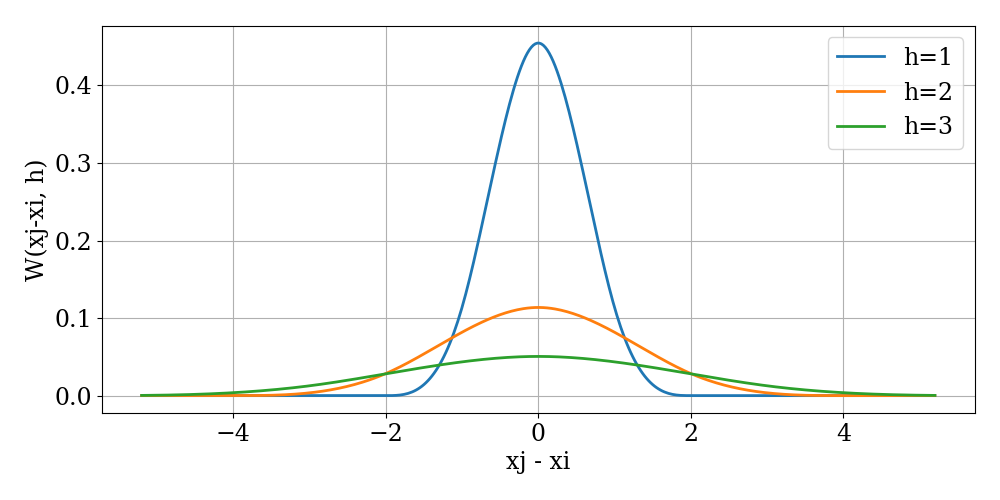
\includegraphics[width=\textwidth]{graphics/KernelPlot.png}
	\caption{TODO}
\end{figure}

Dabei ist \(\alpha\) ein Normalisierungsfaktor, der in verschiedenen Dimensionen wie folgt definiert ist:
1D: \(\alpha = \frac{1}{6h}\), 2D: \(\alpha = \frac{5}{14\pi h^2}\), 3D: \(\alpha = \frac{1}{4\pi h^3}\)

\subsection{Kernel Ableitung}
Die Ableitung der Kernel-Funktion $W_{ij}$ spielt eine entscheidende Rolle bei der Berechnung von Gradienten in der SPH. Sie wird insbesondere zur Berechnung der Druck- und Geschwindigkeitsgradienten verwendet. Die Ableitung der Kernel-Funktion $\nabla_i W_{ij}$ bezüglich der Position des Partikels $i$ ist wie folgt definiert:

\begin{equation*}
	\nabla W(x_j - x_i, h) = \alpha \frac{x_j - x_i}{\|x_j - x_i\|h} 
	\begin{cases} 
	-3(2-\frac{\|x_j - x_i\|}{h})^2 + 12(1-\frac{\|x_j - x_i\|}{h})^2 & 0 \leq \frac{\|x_j - x_i\|}{h} < 1 \\ 
	-3(2-\frac{\|x_j - x_i\|}{h})^2 & 1 \leq \frac{\|x_j - x_i\|}{h} < 2 \\ 
	0 & \frac{\|x_j - x_i\|}{h} \geq 2 
	\end{cases}
\end{equation*}	

\begin{figure}[H]
	\centering
	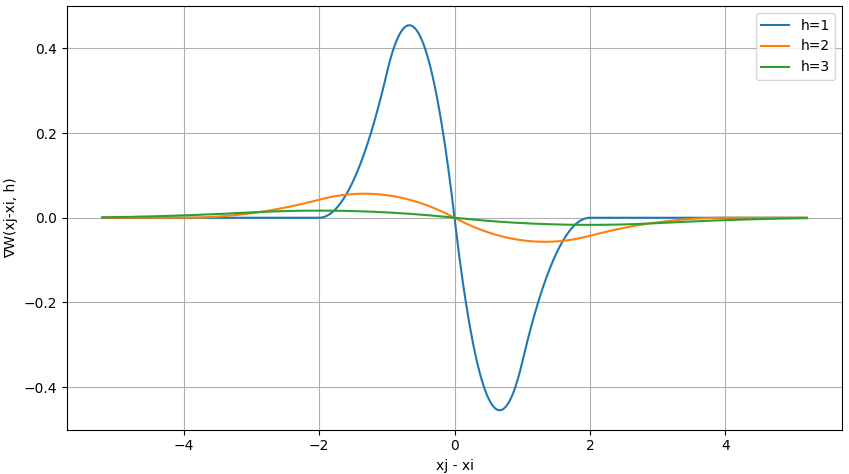
\includegraphics[width=\textwidth]{graphics/KernelDerivPlot.png}
	\caption{TODO}
\end{figure}

Die Kernel-Ableitung ist entscheidend, weil sie in mehreren wichtigen Gleichungen verwendet wird, wie z.B. bei der Berechnung der Kontinuitätsgleichung, der Impulsgleichung, insbesondere bei der Berechnung der Druck- und Viskositätsbeschleunigung.

\subsection{Kontinuitätsgleichung}
Die Kontinuitätsgleichung beschreibt die Erhaltung der Masse und wird in der SPH-Methode wie folgt diskretisiert:
\[
\frac{d\rho_i}{dt} = \sum_j m_j (v_i - v_j) \cdot \nabla_i W_{ij}
\]
Dabei ist \(\rho_i\) die Dichte des Partikels \(i\), \(m_j\) die Masse des Partikels \(j\), \(v_i\) und \(v_j\) die Geschwindigkeiten der Partikel \(i\) und \(j\), und \(\nabla_i W_{ij}\) das Gradientenfeld der Kernel-Funktion bezüglich des Partikels \(i\).

\subsection{Impulsgleichung}
Die Impulsgleichung beschreibt die Erhaltung des Impulses und wird in der SPH-Methode wie folgt diskretisiert:
\[
\frac{d v_i}{dt} = -\sum_j m_j \left( \frac{p_i}{\rho_i^2} + \frac{p_j}{\rho_j^2} \right) \nabla_i W_{ij} + 2 \nu \sum_j \frac{m_j}{\rho_j} \frac{(v_i - v_j) \times (x_i - x_j)}{(x_i - x_j) \times (x_i - x_j) + 0.01\cdot h^2} \nabla_i W_{ij} + f_i
\]

\subsubsection{Druckbeschleunigung}
Die Beschleunigung aufgrund des Drucks wird durch die folgende Gleichung beschrieben:
\begin{equation} \label{equ:druckBesch}
	a_{druck} = -\sum_j m_j \left( \frac{p_i}{\rho_i^2} + \frac{p_j}{\rho_j^2} \right) \nabla_i W_{ij}
\end{equation}
Dabei sind \( p_i \) und \( p_j \) die Drücke der Partikel \( i \) und \( j \), \(\rho_i \) und \(\rho_j \) die Dichten der Partikel \( i \) und \( j \), und \( \nabla_i W_{ij} \) der Gradient der Kernel-Funktion bezüglich des Partikels \( i \).

\subsubsection{Viskositätsbeschleunigung}
Die Beschleunigung aufgrund der Viskosität wird durch die folgende Gleichung beschrieben:
\begin{equation} \label{equ:viskositätBesch}
	a_{viskosität} = 2 \nu \sum_j \frac{m_j}{\rho_j} \frac{(v_i - v_j) \cdot (x_i - x_j)}{(x_i - x_j) \cdot (x_i - x_j) + 0.01\cdot h^2} \nabla_i W_{ij}
\end{equation}
Hier ist \(\nu\) die kinematische Viskosität, \( v_i \) und \( v_j \) sind die Geschwindigkeiten der Partikel \( i \) und \( j \), \( x_i \) und \( x_j \) sind die Positionen der Partikel \( i \) und \( j \), und \(\nabla_i W_{ij}\) ist der Gradient der Kernel-Funktion bezüglich des Partikels \( i \).

\subsubsection{Externe Kräfte}
Die externen Kräfte, die auf ein Partikel wirken, werden durch \( f_i \) dargestellt. Dies kann beispielsweise die Gravitation oder andere externe Einflüsse umfassen:
\begin{equation}
	a_{extern} = f_i
\end{equation}
\subsection{Berechnung der Partikeleigenschaften}
\subsubsection{Dichteberechnung}
Die Dichte jedes Partikels \(i\) wird durch die Summe der Massen der benachbarten Partikel \(j\) gewichtet durch die Kernel-Funktion berechnet:
\begin{equation} \label{equ:localDichte}
	\rho_i = \sum_j m_j W_{ij}
\end{equation}

\subsubsection{Druckberechnung}
Der Druck \(p_i\) wird häufig durch eine Zustandsgleichung berechnet, z.B.:
\begin{equation} \label{equ:lokalDruck}
	p_i = k (\frac{\rho_i}{\rho_0} - 1)
\end{equation}
wobei \(k\) die Steifigkeit Konstante ist und \(\rho_0\) die Ruhe-Dichte.

\section{Simulationsschritt} \label{section_3}
Der Simulationsschritt ist in der SPH Simulation von Zentraler Bedeutung. Dort werden alle nötigen Beschleunigungen ermittelt, die zum simulieren eines Fluides mithilfe von Partikeln, nötigen sind. In diesem Projekt wurde die Methode in 3 Schleifen unterteilt wobei die erste als einzige alle Partikel berücksichtigt. In den Restlichen Schleifen werden nur Partikel welche das Fluid bilden beachtet und Partikel zum Simulieren der Grenze Ignoriert.

Eigenschaften wie die Partikelgröße und die Ruhedichte der Flüssigkeit werden vor dem Starten der Simulation festgelegt. Aus diesen wird eine Masse für die Partikel ermittelt welche im laufe der Simulation konstant bleibt. Weitere Werte werden im Kapitel TODO erläutert. 

Darauf hin werden in der ersten Schleife die restlichen locale Eigenschaften ermittelt. Dazu müssen die Nachbar Partikel in einem Radius $2 \cdot Partikelgröße$ um die Partikel ermittelt werden. Mit Hilfe der Nachbarn wird die Lokale Dichte und der Lokale Druck jedes Partikels bestimmt. Diese werden für die Berechnungen der nächste Schleife benötigt. In dieser werden, für alle Partikel die das Fluid bilden, die Viskosität- und Druckbeschleunigungen berechnet.
Anhand dieser Beschleunigungen werden die Positionen der Partikel in der letzten schleife Aktualisiert. 

\begin{algorithm}[H]
\caption{Simulationsschritt}
\begin{algorithmic}[1]
\State \textbf{For each} particle \textbf{in} particles
\State \quad $\text{FindNeighbors()}$
\State \quad $\text{ComputeLocalDensity()}$ \hfill \eqref{equ:localDichte}
\State \quad $\text{ComputeLocalPressure()}$ \hfill \eqref{equ:lokalDruck}
\vspace{1em}
\State \textbf{For each} particle \textbf{in} noBoundaryParticles
\State \quad $\text{GetViscosityAcceleration}()$ \hfill \eqref{equ:viskositätBesch}
\State \quad $\text{GetPressureAcceleration}()$ \hfill \eqref{equ:druckBesch}
\vspace{1em}
\State \textbf{For each} particle \textbf{in} noBoundaryparticles
\State \quad $\text{acceleration} = \text{viscosityAcceleration} + \text{pressureAcceleration} + \text{gravitation}$
\State \quad $\text{particle.Velocity} += \text{timeSteps}\;\cdot\;\text{acceleration}$
\State \quad $\text{particle.Position} += \text{timeSteps}\;\cdot\;\text{particle.Velocity}$
\end{algorithmic}
\end{algorithm}

\section{Nachbarschaft Suche} \label{section_4}
Die Nachbarschaft Suche ist das Fundament der Simulation. Diese erlaubt das ermitteln der Nachbar Partikel in einem feste Radius um eine Position zum Berechnen lokaler Werte. Ein naiver Ansatz wäre, für alle Partikel den Abstand zur Position zu ermitteln und zu prüfen ob sich diese im Radius zu befinden. Diese Methode weist jedoch eine quadratische Laufzeitkomplexität auf, da für jedes Partikel der Abstand zu allen anderen Partikeln berechnet werden muss. Dies führt zu einer Laufzeit von $O(n^2)$, wobei $n$ die Anzahl der Partikel ist. Bei großen Partikelzahlen wird dieser Ansatz daher ineffizient und rechenintensiv.

Für das Projekt wurde dementsprechend das Räumliche Hashing verwendet. Dabei handelt es sich um eine Datenstruktur die den Raum in einzelne Blöcke unterteilt. Beim ermitteln von Nachbar Partikel müssen dadurch nicht mehr alle Partikel geprüft werden sondern nur diese die sich in dem selbem Block oder Nachbar Block befinden. Dies führt zu einer effizienteren und weniger rechenintensiven Methode zum bestimmen der Nachbarn.

\subsection{Einfügen von Partikel}
Um ein Partikel in die Datenstruktur einzufügen wird als erst ein Hashwert bezüglich der Position errechnet. Dazu wird der Position Vektor durch die Blockgröße geteilt und das Ergebnis abgerundet.
\begin{algorithm}[H]
	\caption{Hash Funktion}
	\begin{algorithmic}[1]
		\Require Vector $\mathbf{v} = (v_x, v_y)$, scalar $\text{CellSize}$
		\Ensure Hashed vector $\mathbf{h} = (h_x, h_y)$
		\State $\mathbf{h} \leftarrow \frac{\mathbf{v}}{\text{CellSize}}$
		\State $\mathbf{h} \leftarrow \lfloor \mathbf{h} \rfloor$
		\Return $\mathbf{h}$
	\end{algorithmic}
\end{algorithm}

Schließlich wird der Partikel in eine Liste innerhalb der Hashtabelle Eingefügt. Das löschen eines Partikels aus der Datenstruktur funktioniert Analog.

\subsection{Updaten der Partikel Positionen}
Wurden die Positionen der Partikel im Simulationsschritt aktualisiert müssen ebenfalls die Einträge in der Hashtabelle Aktualisiert werden. Dazu werden die Partikel vor dem Aktualisieren der Position aus der Datenstruktur entfernt und nach der Aktualisierung wieder eingefügt. 

\subsection{Ermitteln von Nachbarn}
Das ermitteln von Nachbar Partikel ist das Fundament des Simulationsschrittes. Zu erst werden die Blöcke, welche Teil des Radiuses sind und somit durchsucht werden müssen, ermittelt. Des weiterem werden die Partikel in den Blöcke überprüft ob sich diese in dem Radius um die Position befinden.
\begin{algorithm}[H]
    \caption{Partikel im Radius}
    \begin{algorithmic}[1]
		\Require Position $\mathbf{p}$, Radius $r$
        \Ensure Liste der Partikel im Radius: $\text{partikelImRadius}$
        \State $startX \leftarrow \lfloor (\mathbf{p}_x - r) / \text{CellSize} \rfloor$
        \State $endX \leftarrow \lceil (\mathbf{p}_x + r) / \text{CellSize} \rceil$
        \State $startY \leftarrow \lfloor (\mathbf{p}_y - r) / \text{CellSize} \rfloor$
        \State $endY \leftarrow \lceil (\mathbf{p}_y + r) / \text{CellSize} \rceil$
        \For{($x \leftarrow startX$ \textbf{to} $endX$)}
            \For{($y \leftarrow startY$ \textbf{to} $endY$)}
                \If{($(x , y)$ existiert in $\text{Hashtabelle}$)}
                    \ForAll{(Partikel in \text{Hashtabelle}[hash])}
                        \If{($\text{Distance}(Partikel.\text{Position}, \mathbf{p}) \leq r$)}
                            \State $\text{partikelImRadius}.\text{add}(q)$
                        \EndIf
                    \EndFor
                \EndIf
            \EndFor
        \EndFor
        \Return $\text{partikelImRadius}$
    \end{algorithmic}
\end{algorithm}
Dies erlaubt es die Anzahl an Partikel welche überprüft werden müssen zu beschränken und die Laufzeit zu verringern. 

\section{Implementierung} \label{section_5}
Die Implementierung ist zentraler Bestandteil des Projektes. Implementiert wurde in C\# mit Hilfe des Frameworks Monogame. In diesem Kapitel wird die Implementierung von Tests, essenziell für die Korrektheit der Simulation, und die Implementierung Spezieller Hilfsmittel vorgestellt. 

\subsection{Tests}
Das Testen der einzelnen Komponenten des Simulationsschrittes sind essenziell für die Funktionalität und Korrektheit der Simulation. Sie helfen dabei offensichtliche Probleme in der Simulation zu isolieren und zu Korrigieren. Allerdings sind ebenfalls nicht offensichtliche Fehler in der Simulation nicht auszuschließen, weshalb die Test ebenfalls zusätzliche Sicherheit garantieren. Diese werden beim Starten der Simulation gestartet. Dabei wird ein Ideales Gitter der Größe  $10 \cdot 10$  mit Partikel erzeugt. Ideale bedeutet dass alle Partikel den gleichen Abstand h zueinander haben. Auf diesen Partikeln werden schließlich die Tests angewendet. Schlägt ein Test fehl erscheint eine Nachricht in Roter Schrift auf dem Bildschirm. 

Das Fundament aller Berechnungen ist die Nachbarschafts Suche. Ausschließlich bei diesem Test wird ein kleineres Ideales Gitter mit $5 \cdot 5$ Partikeln erzeugt. Um zu gewährleisten dass alle Partikel, die sich im Such-Radius um den mittleren Partikel befinden, gefunden werden, werden die von der Räumlichen Datenstruktur gefunden Partikeln in einer Liste gesammelt. Die Anzahl der Partikel in der Liste muss nach dem suchen 13 ergeben.

Für die folgenden Tests werden für alle Partikel aus dem größerem Gitter die Nachbarn gesucht und die Komponenten getestet. 
Begonnen wird mit der Kernel Funktion. Eine falsche Gewichtung der Nachbarn in den Berechnungen führt zu falschen Kräften und Bewegungen der Teilchen. Um die Funktionalität der Kernel Funktion zu gewährleisten werden vier Test auf diese angewandt. Der erste Test beruht auf der Eigenschaft \eqref{kernelEigenschaft1}. Dabei wird der Wert der Kernel-Funktion für ein Ideales Gitter an Nachbarn berechnet, welcher eins ergeben soll. Des weiterem werden noch 3 Tests ohne das Gitter durchlaufen. Für eine relative Partikel Entfernung $q= \frac{0}{1} = 0$ und $q = \frac{1}{1} = 1$ ergeben die Werte der Kernel Gleichung $W(1, 0) = 4 * \alpha$ und $W(1, 1) = \alpha$ wobei $\alpha$ der Normalisierungsfaktor der Kernel-Funktion ist. 
\[W(0) = \alpha ((2-0)^3 - 4(1-0)^3) = \alpha (8 - 4) = 4\alpha\]
\[W(1) = \alpha ((2-1)^3) = \alpha\]
Zuletzt wird die Kernel Eigenschaft \eqref{kernelEigenschaft5} geprüft. Dabei muss $W = 0$ für eine Partikel Entfernung größer $2h$ sein.
Weiterhin wird die Funktionalität der Kernel Ableitung getestet. Diese ist ein Wesentlicher Bestandteil der Gleichungen zum berechnen der wirkenden Kräfte auf die Partikel. Auf dieser Komponente werden sieben Tests angewandt. TODO

\subsection{Tools}
Die simulation verfügt über einige implementierte Tools zur Steuerung der Simulation. Durch drücken der Taste \keys{H} öffnet sich eine Liste von Aktionen zum Steuern der Simulation. Einige der Wichtigsten Aktionen werden in diesem Unterkapitel vorgestellt. 

Die Simulation verfügt über mehrere Verschiedene \glqq Szenarios\grqq{}. Ein \glqq Szenarios\grqq{} bedeutet hier, ein Box oder andere Geometrische Form, welche eine Barriere für die zu simulierenden Flüssigkeit bildet. Diese können mit der Taste \keys{V} gewechselt werden. Durch wechseln der Szene oder Drücken der Taste \keys{del} werden alle Partikel der Szene gelöscht. 

Ebenfalls können, zum Zwecke der Simulation, Partikel mit Hilfe der Maus in der jeweiligen Szene platziert werden. Dazu wird mit der Taste \keys{Q} die Form einer Box, eines Kreises oder eines einzelnes Partikel
ausgewählt. Im Falle der Box und des Kreises können die Höhe und Breite mit den Tasten \keys{W}, \keys{S} und \keys{D}, \keys{A} verändert werden. Platziert werden die Partikel durch linkes Klicken der Maus.

Im sinne der Analyse können durch drücken der Taste \keys{F2} Daten gesammelt werden und durch drücken von \keys{F1} gespeichert werden. Zusätzlich wird durch drücken der Taste \keys{F12} ein Screenshot aufgenommen. Gespeichert werden alle Dateien im Dokumenten Ordner des Benutzers.

\section{Analysen} \label{section_6}
Zuletzt werden in diesem Kapitel die gesammelten Daten von Experimenten visualisiert und Vorstellen. Die Experimente befassen sich mit Schwerpunkte der Simulation. Das erste Experiment beobachtet die Auswirkung der Einstellungsparameter auf die Stabilität und das Verhalten des Fluiden. Dazu wird eine Wassersäule simuliert und das Verhalten der Dichte aller Partikel zu analysieren. Da der Druck innerhalb eines Fluiden Abhängig der Gravitation, Fluid Höhe und Fluid Dichte ist, reicht es hier eine schmale Säule für das Experiment zu nutzen. 
Zunächst wird der Einfluss der Beschleunigung Nachbarschafts Suche auf die Performance der Simulation betrachtet. Hierfür wird die Zeit um einen Simulationsschritt zu durchlaufen (Simulationsschrittzeit) beobachtet. Dabei wird die Anzahl an Partikel kontinuierliche erhöht und in Relation zur Simulationsschrittzeit gesetzt. Dieses Vorgehen wird auf beide Methoden der Nachbarschafts Suche angewandt.
Analog dazu wird ebenfalls betrachtet, wie sich die Performance verhält für eine Sequentielle- und Parallele Prozessverarbeitung.

\subsection{Säulenexperiment}

\begin{wrapfigure}{r}{.39\textwidth}
	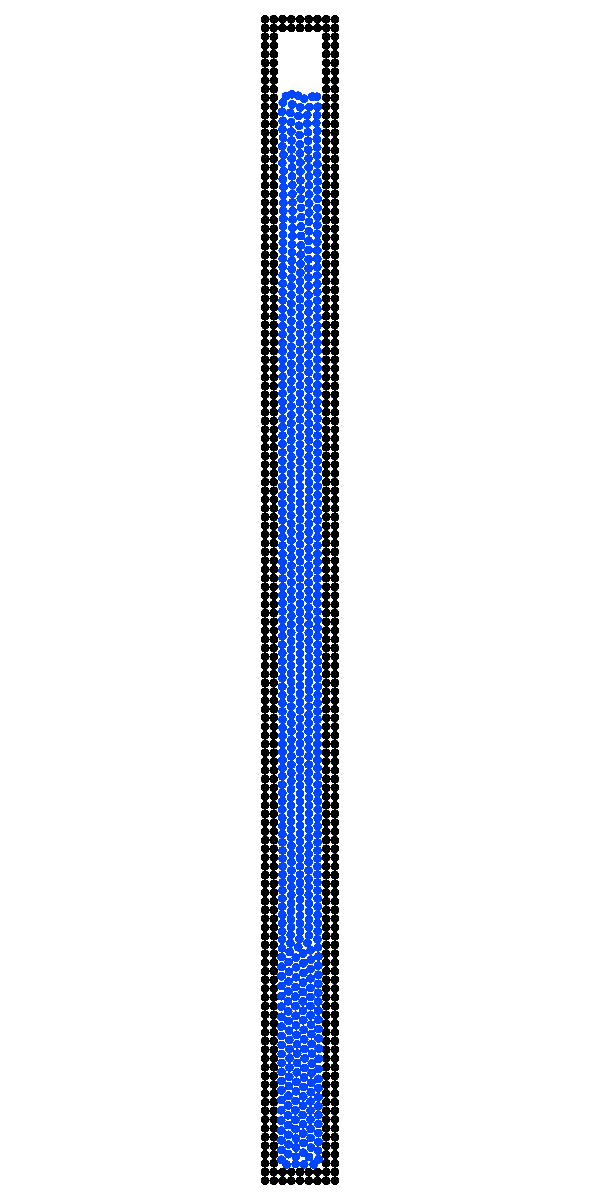
\includegraphics[width=\linewidth]{graphics/20240813135808.png} 
	\caption{Säulenexperiment}
	\label{Säulenexperiment}
\end{wrapfigure}

Beim Säulenexperiment (siehe Abbildung \ref{Säulenexperiment}) wurde die Auswirkung der Steifigkeit $k$, der Viskosität $\nu$ und des Zeitschrittes $\Delta t$ auf die locale Dichten aller Partikel beobachtet. Dazu wurde für jeden Simulationsschritt der Mittelwert der Dichten aller Partikeln ermittelt und im Verhältnis der Simulationsschritte oder der Zeit dargestellt. Der wichtigste Parameter ist hierbei der Steifigkeit Parameter. Dieser ist ein Skalar für die Berechnung des der Lokalen Dichte \eqref{equ:localDichte} und hat direkten Einfluss auf die Druckbeschleunigungen \eqref{equ:druckBesch}. 

In Abbildung \ref{Säulenexperiment_k} wurde die Säule mit verschiedenen Werten für $k$ simuliert. Bemerkbar ist, dass die lokale Dichte konstant bleibt und sich der Dichtefehler für steigendes $k$ minimiert. Die lokale Dichte konvergiert dabei in Richtung der Flüssigkeitsdichte. Somit ist $k$ ein Skalar für die Kompressibilität des Fluiden.
Um die Visualisierung anschaulicher zu gestalten wurde für dieses Experiment eine hohe Viskosität gewählt. Dadurch werden Schwankungen des Dichtefehler minimiert, was zu einem Konstanten Wert führt. 

Im Zweitem Säulenexperiment wurde die Viskosität $\nu$ variiert. Diese kontrolliert wie stark ein Partikel von seinen Nachbarn gedämpft wird. In Abbildung \ref{Säulenexperiment_v} wird dargestellt wie die Viskosität die Schwankungen der lokalen Dichte Dämpft. Dies Zeigt sich durch ein verringern der Amplitude. Umso größer die Viskosität, umso stärker kleben die Partikel aneinander. 

Der letzte Parameter ist der Zeitschritt. Dieser skaliert die Beschleunigung auf das Partikel und ebenfalls den Bewegungsschritt des Partikeln. In Abbildung \ref{Säulenexperiment_t} ist auffällig wie sich mit kleinerem $\Delta t$ die Amplitude vergrößert und die Frequenz vergrößert. Dass die Frequenz sich vergrößert ist trivial da die Bewegung des Partikel gebremst wird und sich die Schritte der Partikel sich für ein Simulationsschritt verkleinert haben. 

\begin{figure}[H]
	\centering
	\subfigure[Säulenexperiment mit Verschiedener Steifigkeit k]
	{
		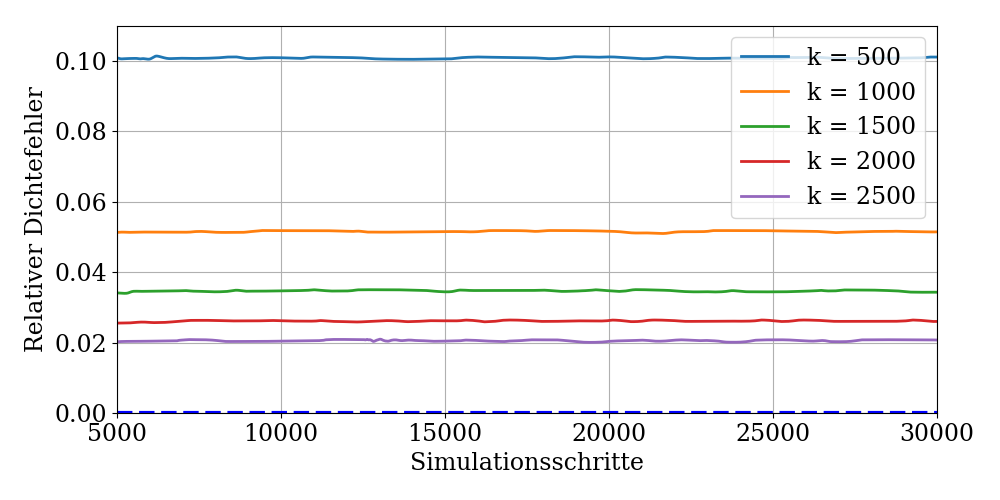
\includegraphics[width=.9\textwidth]{graphics/Steifigkeit.png}	
		\label{Säulenexperiment_k}
	}
	\subfigure[Säulenexperiment mit Verschiedener Viskosität v]
	{
		\includegraphics[width=.9\textwidth]{graphics/Viskosität.png}	
		\label{Säulenexperiment_v}
	}
	\subfigure[Säulenexperiment mit Verschiedenen Zeitschritten $\Delta$ t]
	{
		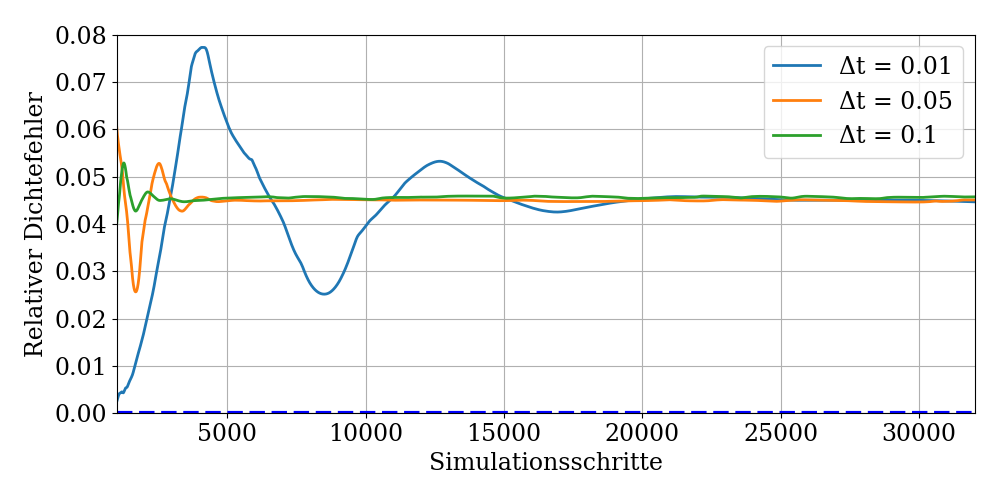
\includegraphics[width=.9\textwidth]{graphics/Zeitschritt.png}	
		\label{Säulenexperiment_t}
	}
	\caption{Säulenexperiment mit verschiedenen Einstellungsparameter}
\end{figure}
% Larger stiffness -> less compressibility -> smaller time step 

\subsection{Nachbarschafts Suche}
\begin{figure}[H]
	\centering
	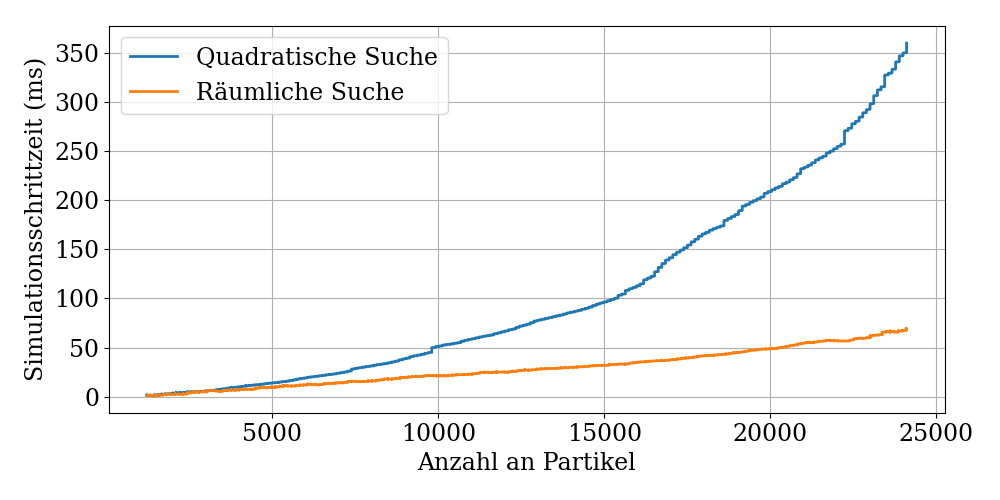
\includegraphics[width=\textwidth]{graphics/Nachbarschafts-Suche.png}
	\caption{Nachbarschafts-Suche}
\end{figure}

\subsection{Prozessverarbeitung}
\begin{figure}[H]
	\centering
	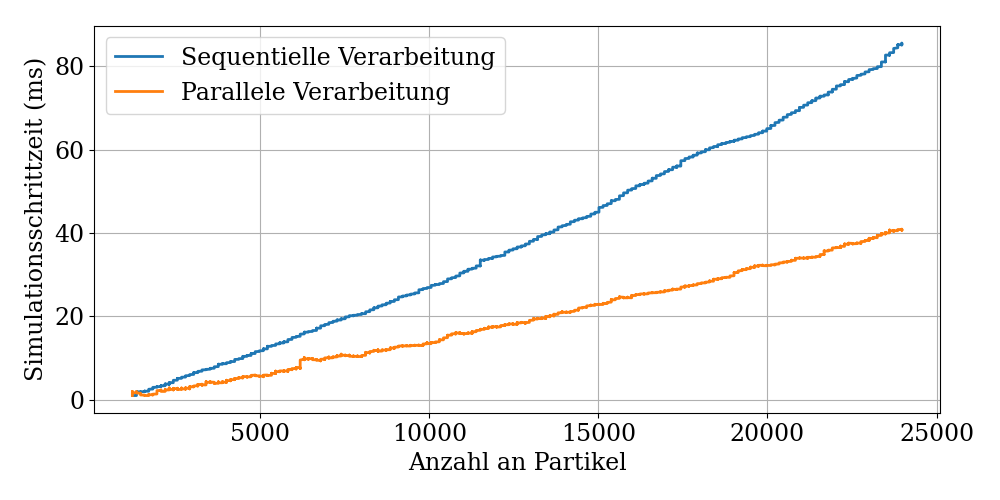
\includegraphics[width=\textwidth]{graphics/Prozessverarbeitung.png}
	\caption{Prozessverarbeitung}
\end{figure}

\section{Schlussfolgerung}

\section{Bibliographie}
\end{document}